\begin{frame}{Распределение интенсивности МК когерентностей ЯМР}
\begin{columns}
  \column{0.4\textwidth}
  \vspace{-3mm}
  \begin{figure}
    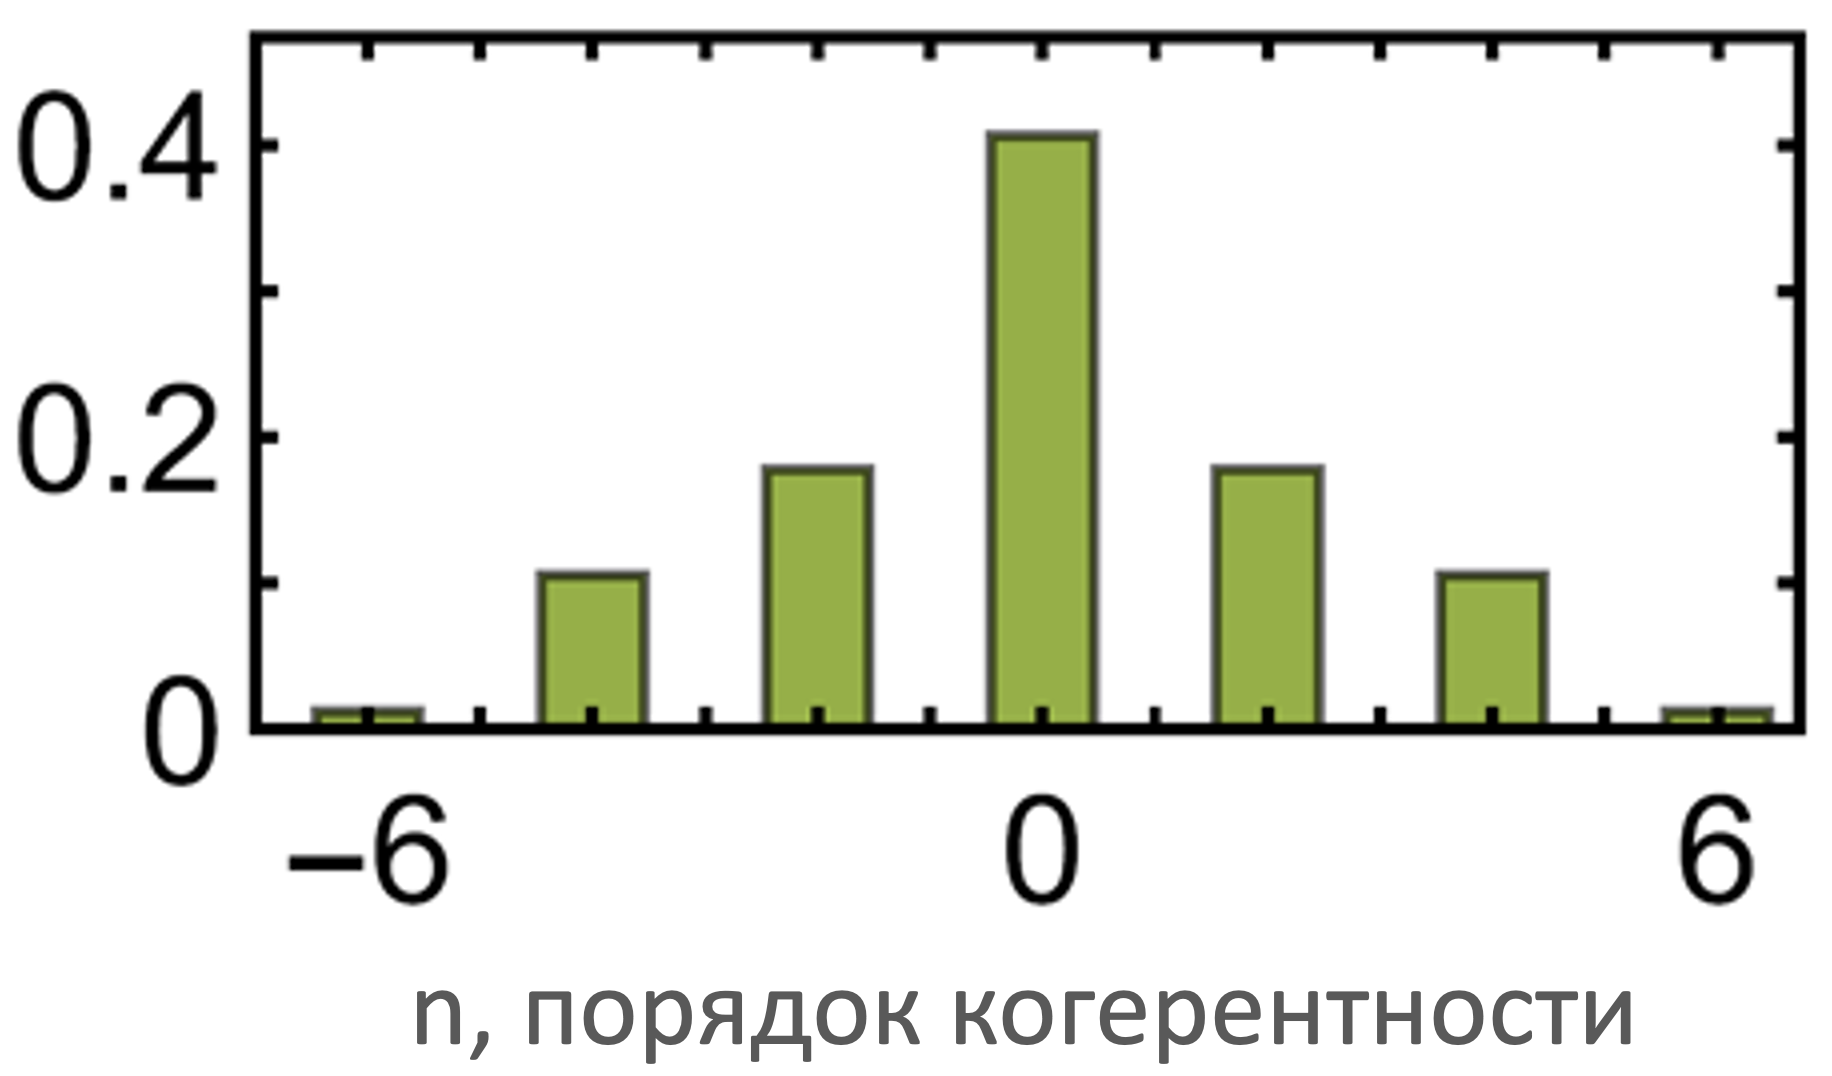
\includegraphics[width=\textwidth]{mq-coherence-intensities-hist.png}
    \caption{Распределение интенсивности МК когерентностей ЯМР.}
  \end{figure}

    \column{0.5\textwidth}
    \begin{block}{}
      Второй момент (дисперсия) распределения МК когерентностей ЯМР.
      $$
        M_2 (\tau,\beta) = \sum_n n^2 J_n(\tau,\beta)
      $$
      где $J_n$ интенсивность МК когерентности ЯМР порядка $n$.
    \end{block}

\end{columns}
\end{frame}
\note{
  Подсчитать информацию фишера не просто подсчитить но она связана с рейльной физической величеной.
  Важно отметить что здесь нам удалось связать меру информации с физической величиной.
  Под действием гамильтониана происходят переходы между энергетическими уровнями
  и возникаюм многоквантовые когерентности.
  Гистограма показывает частоту этих переходов.
  ЯМР отличный инструмент и наша работа это подтверждает.

  % mq-coherences-distribution % JETP 2018
}
